\documentclass[
handout,
aspectratio=169]{beamer}
\usetheme{default}

\usepackage{tikz}

\usepackage{amsmath,amssymb}

\newcommand{\pitem}{\pause\item}

\newtheorem{statement}{Statement}

\newcommand{\bits}{\{0,1\}}
\newcommand{\bitstr}{\bits^*}
\newcommand{\sshalf}{{\textstyle\frac12}}
\newcommand{\seqn}[2]{{#1}_1,{#1}_2,\dotsc,{#1}_{#2}}
\newcommand{\seqin}[3]{{#1}_{{#2}_1},{#1}_{{#2}_2},\dotsc,{#1}_{{#2}_{#3}}}
\newcommand{\IC}{\mathrm{IC}}
\newcommand{\poly}{\mathrm{poly}}
\newcommand{\Nat}{\mathbb{N}}

\DeclareMathOperator{\dom}{dom}
\DeclareMathOperator{\rank}{rank}
\DeclareMathOperator{\rng}{rng}
\DeclareMathOperator*{\E}{\mathbb{E}}

\newenvironment{sol}{%
    \begin{block}{}%
        \setbeamercolor{block body}{bg=lightgray}%
    }{
\end{block}}

\AtBeginSection[]{
    \begin{frame}
        \vfill
        \centering
        \begin{beamercolorbox}[sep=8pt,center,shadow=true,rounded=true]{title}
            \usebeamerfont{title}\insertsectionhead\par%
        \end{beamercolorbox}
        \vfill
    \end{frame}
}


\title{Cryptography}
\author{Alexander Smal at NUP}
\date{13.11.2024.\\ Lecture 4}

\begin{document}
%%%%%%%%%%%%%%%%%%%%%%%%%%%%%%%%%%%%%%%%%%%%%%%%%%%%%%%%%%%%%%%%%%%%%%%%
\begin{frame}[plain]
    \maketitle
\end{frame}
%%%%%%%%%%%%%%%%%%%%%%%%%%%%%%%%%%%%%%%%%%%%%%%%%%%%%%%%%%%%%%%%%%%%%%%%

\section{Symmetric Key Encryption}
%%%%%%%%%%%%%%%%%%%%%%%%%%%%%%%%%%%%%%%%%%%%%%%%%%%%%%%%%%%%%%%%%%%%%%%%
\begin{frame}{Symmetric Key Encryption}
    \begin{itemize}
        \item
    We will assume that the computational resources of the adversary are unlimited.

        \pitem
    We encrypt a message $m$ with an encryption key $k$.

        \pitem As a result, we get the \emph{ciphertext} $c = E(k, m)$.


        \pitem The recipient of the ciphertext also knows the key $k$ and can decipher the original message $m = D(k, c)$.

        \pitem We assume that $m$ and $k$ are random variables.

        \pitem The adversary does not know $m$ and $k$, but knows $c$.

        \pitem For a \emph{perfect} encryption scheme, the following conditions must hold:
        \[
        \begin{cases}
            H(c \mid k, m) = 0,\\
            H(m \mid k, c) = 0,\\
            I(c : m) = 0.
        \end{cases}
        \]

    \end{itemize}

\end{frame}
%%%%%%%%%%%%%%%%%%%%%%%%%%%%%%%%%%%%%%%%%%%%%%%%%%%%%%%%%%%%%%%%%%%%%%%%

%%%%%%%%%%%%%%%%%%%%%%%%%%%%%%%%%%%%%%%%%%%%%%%%%%%%%%%%%%%%%%%%%%%%%%%%
\begin{frame}{Perfect Secrecy}
    \begin{theorem}[Shannon]
        $H(k) \ge H(m)$, even if $H(c \mid k, m) > 0$ (i.e., the algorithm $E$ uses randomness).
    \end{theorem}
    Note that a one-time pad has this property.
    \pause
    \begin{proof}
        According to the condition, $x + w = 0$, i.e., $x = -w$.

        \begin{center}
            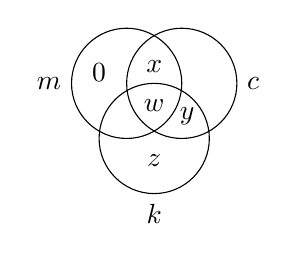
\begin{tikzpicture}[scale=0.7]
                \tikzstyle{circ}=[circle, draw, inner sep=0pt, minimum width=1.4cm]

                \node[circ, label=left:$m$]  (x) at (1,1) {};
                \node[circ, label=right:$c$] (y) at (2,1) {};
                \node[circ, label=below:$k$] (z) at (1.5,0) {};
                \node at (0.5,1.2) {$0$};
                \node at (1.5,-.4) {$z$};

                \node at (1.5,1.3) {$x$};
                \node at (2.1,0.4) {$y$};

                \node at (1.5,0.6) {$w$};
            \end{tikzpicture}
        \end{center}
        Since the mutual information is non-negative, we have $w + y \ge 0$, i.e.,
        $y \ge -w = x$. Now, from $y \ge x$ and $z \ge 0$, it follows that $H(k) \ge H(m)$.
    \end{proof}
\end{frame}
%%%%%%%%%%%%%%%%%%%%%%%%%%%%%%%%%%%%%%%%%%%%%%%%%%%%%%%%%%%%%%%%%%%%%%%%

\section{Secret Sharing Schemes}
%%%%%%%%%%%%%%%%%%%%%%%%%%%%%%%%%%%%%%%%%%%%%%%%%%%%%%%%%%%%%%%%%%%%%%%%
\begin{frame}{Secret Sharing Schemes}
    We want to share some secret $S_0$ among $n$ participant in such a way that they can only use it together, while any subset of participants cannot.

    \begin{definition}
        A \emph{perfect secret sharing scheme} is a joint distribution of probabilities $(S_0, \seqn{S}{n})$ such that
        \[
        \begin{cases}
            H(S_0 \mid \seqn{S}{n}) = 0,\\
            H(S_0 \mid \seqin{S}{i}{k}) = H(S_0), & k < n.
        \end{cases}
        \]
        The second condition can be rewritten as $I(S_0 : \seqin{S}{i}{k}) = 0$.
    \end{definition}
\end{frame}
%%%%%%%%%%%%%%%%%%%%%%%%%%%%%%%%%%%%%%%%%%%%%%%%%%%%%%%%%%%%%%%%%%%%%%%%

%%%%%%%%%%%%%%%%%%%%%%%%%%%%%%%%%%%%%%%%%%%%%%%%%%%%%%%%%%%%%%%%%%%%%%%%
\begin{frame}{Construction}
    \begin{itemize}
        \item Let us assume that $S_0$ is encoded using $\ell$ bits.
        \pitem We independently and uniformly choose $S_1, \dotsc, S_{n-1} \in \{0,1\}^\ell$.
        \pitem $S_n$ is determined by the condition $S_0 \oplus S_1 \oplus S_2 \oplus \dotsb \oplus S_n = \vec 0$.
    \end{itemize}

    \pause
    \begin{theorem}
        This secret sharing scheme is perfect.
    \end{theorem}

\end{frame}
%%%%%%%%%%%%%%%%%%%%%%%%%%%%%%%%%%%%%%%%%%%%%%%%%%%%%%%%%%%%%%%%%%%%%%%%

%%%%%%%%%%%%%%%%%%%%%%%%%%%%%%%%%%%%%%%%%%%%%%%%%%%%%%%%%%%%%%%%%%%%%%%%
\begin{frame}{Threshold Secret Sharing Schemes}
\begin{definition}
    A \emph{threshold perfect secret sharing scheme} is a joint distribution of probabilities $(S_0, \seqn{S}{n})$ such that
    \[
    \begin{cases}
        H(S_0 \mid \seqin{S}{i}{t}) = 0,\\
        H(S_0 \mid \seqin{S}{i}{k}) = H(S_0), & k < t.
    \end{cases}
    \]
\end{definition}


\end{frame}
%%%%%%%%%%%%%%%%%%%%%%%%%%%%%%%%%%%%%%%%%%%%%%%%%%%%%%%%%%%%%%%%%%%%%%%%

%%%%%%%%%%%%%%%%%%%%%%%%%%%%%%%%%%%%%%%%%%%%%%%%%%%%%%%%%%%%%%%%%%%%%%%%
\begin{frame}{Shamir's Threshold Scheme}
    \begin{itemize}
    \item Let us assume that the secret $S_0$ is an element of some finite field $\mathbb{F}_q$.

    \pitem Choose a random polynomial $p$ over the field $\mathbb{F}_q$ of degree at most $t-1$: choose $t-1$ coefficients independently and uniformly,

    \pitem determine the last (constant) coefficient from the condition $p(0) = S_0$.

    \pitem Randomly select a set of distinct non-zero elements of the field $\seqn{a}{n} \in \mathbb{F}_q$,

    \pitem Compute the participants' secrets as the value of the polynomial at the corresponding points $S_i = p(a_i)$.

    \pitem Any $t$ participants can use polynomial interpolation, and compute $S_0 = p(0)$.

    \pitem Any $t' < t$ participants have no information about $S_0$.
    \end{itemize}

    \pause
    \begin{theorem}
        Shamir's threshold scheme is perfect.
    \end{theorem}
    \pause
    \begin{proof}
        Any polynomial of degree less than $t-1$ can be extended to a polynomial of higher degree with any value at point $0$.
        \end{proof}	\end{frame}
%%%%%%%%%%%%%%%%%%%%%%%%%%%%%%%%%%%%%%%%%%%%%%%%%%%%%%%%%%%%%%%%%%%%%%%%

%%%%%%%%%%%%%%%%%%%%%%%%%%%%%%%%%%%%%%%%%%%%%%%%%%%%%%%%%%%%%%%%%%%%%%%%
\begin{frame}{Secret Sharing Schemes for Access Structures}
    A \emph{perfect secret sharing scheme for an access structure $\Gamma \subset 2^{[n]}$} (with $\Gamma$ being upward closed) is a joint distribution of probabilities $(S_0, \seqn{S}{n})$ such that
    \[
    \begin{cases}
        H(S_0 \mid \seqin{S}{i}{m}) = 0, & \{\seqn{i}{m}\} \in \Gamma,\\
        H(S_0 \mid \seqin{S}{i}{m}) = H(S_0), & \{\seqn{i}{m}\} \not\in \Gamma.
    \end{cases}
    \]

    An \emph{ideal secret sharing scheme} is a perfect secret sharing scheme with the additional requirement of ``efficiency'':
    $
    \forall i \in \{1, 2, \dotsc, n\},\ H(S_i) \le H(S_0).
    $

\begin{theorem}
    If participant $i$ is \emph{essential} in the access structure $\Gamma$ (i.e., there exists
    some $s \in \Gamma$ such that $s \setminus \{i\} \not\in \Gamma$), then $H(S_i) \ge H(S_0)$.
\end{theorem}

Note that Shamir's scheme is ideal.

\end{frame}
%%%%%%%%%%%%%%%%%%%%%%%%%%%%%%%%%%%%%%%%%%%%%%%%%%%%%%%%%%%%%%%%%%%%%%%%

%%%%%%%%%%%%%%%%%%%%%%%%%%%%%%%%%%%%%%%%%%%%%%%%%%%%%%%%%%%%%%%%%%%%%%%%
\begin{frame}{Theorem about Essential Participants}
    \begin{theorem}
        If participant $i$ is \emph{essential} in the access structure $\Gamma$, then $H(S_i) \ge H(S_0)$.
    \end{theorem}

    \begin{proof}
        Let $s=\{i, \seqn{j}{k}\} \in \Gamma$, and $s \setminus \{i\} \not\in \Gamma$.\\
        Denote $h = I(S_0 : \seqin{S}{j}{k} \mid S_i)$,
        and $g = I(S_i : \seqin{S}{j}{k} \mid S_0)$.\\
        $I(S_0 : \seqin{S}{j}{k}) = 0\ \implies\ I(S_0 : S_i : \seqin{S}{j}{k}) = -h$.\\
        Similarly, $I(S_i : \seqin{S}{j}{k}) \ge 0 \ \implies\ g \ge h$.

        \begin{center}
            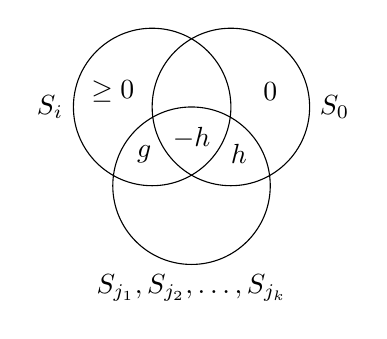
\begin{tikzpicture}
                \tikzstyle{circ}=[circle, draw, inner sep=0pt, minimum width=2cm]

                \node[circ, label=left:$S_i$]  (a) at (1,1) {};
                \node[circ, label=right:$S_0$]  (b) at (2,1) {};
                \node[circ, label=below:$\seqin{S}{j}{k}$] (c) at (1.5,0) {};
                \node at (0.5,1.2) {$\ge 0$};
                \node at (2.5,1.2) {$0$};

                \node at (2.1,0.4) {$h$};
                \node at (0.9,0.4) {$g$};

                \node at (1.5,0.6) {$-h$};
            \end{tikzpicture}
        \end{center}
        Thus, $H(S_i) \ge H(S_0)$.
    \end{proof}

\end{frame}
%%%%%%%%%%%%%%%%%%%%%%%%%%%%%%%%%%%%%%%%%%%%%%%%%%%%%%%%%%%%%%%%%%%%%%%%

%%%%%%%%%%%%%%%%%%%%%%%%%%%%%%%%%%%%%%%%%%%%%%%%%%%%%%%%%%%%%%%%%%%%%%%%
\begin{frame}{Perfect Secret Sharing Schemes}
        Previous theorem shows that there cannot be a more ``efficient'' secret sharing scheme than an ideal one.

    \begin{statement}
        For any access structure $\Gamma$, there exists a perfect secret sharing scheme.
    \end{statement}

    \begin{proof}
        Let us create a separate set of secrets $S^A_{i_1}, S^A_{i_2}, \dotsc, S^A_{i_k}$ for each subset
        $A = \{\seqn{i}{k}\} \in \Gamma$: $S^A_{i_1} \oplus S^A_{i_2} \oplus \dotsb \oplus S^A_{i_k} = S_0$.
        (It is sufficient to consider only minimal sets $A$.)
    \end{proof}

        The proposed scheme is not ideal.


\end{frame}
%%%%%%%%%%%%%%%%%%%%%%%%%%%%%%%%%%%%%%%%%%%%%%%%%%%%%%%%%%%%%%%%%%%%%%%%

%%%%%%%%%%%%%%%%%%%%%%%%%%%%%%%%%%%%%%%%%%%%%%%%%%%%%%%%%%%%%%%%%%%%%%%%
\begin{frame}{Ideal Secret Sharing Schemes}
    \begin{theorem}
        There exist access structures for which there is no ideal secret sharing scheme.
    \end{theorem}

    Consider the access structure defined by the following graph (the edges correspond to the authorized
    sets).
    \begin{center}
        \begin{tikzpicture}
            \tikzstyle{vert}=[circle, draw, fill=black!50,
            inner sep=0pt, minimum width=4pt]
            \node at (0,0.5) {};
            \foreach \i/\n in {1/a, 2/b, 3/c, 4/d}
            \node[vert, label=below:\i] (\n) at (\i,0) {};

            \path (a) edge (b);
            \path (b) edge (c);
            \path (c) edge (d);
        \end{tikzpicture}
    \end{center}
    We will show that, $H(S_2) + H(S_3) \ge 3H(S_0)$, i.e.,
    $\max_i \frac{H(S_i)}{H(S_0)} \ge \frac{3}{2}$.

    For the proof, we will need three lemmas.

    Let us denote $h = H(S_0)$.
\end{frame}
%%%%%%%%%%%%%%%%%%%%%%%%%%%%%%%%%%%%%%%%%%%%%%%%%%%%%%%%%%%%%%%%%%%%%%%%

%%%%%%%%%%%%%%%%%%%%%%%%%%%%%%%%%%%%%%%%%%%%%%%%%%%%%%%%%%%%%%%%%%%%%%%%
\begin{frame}{Ideal Secret Sharing Schemes: Lemma 1}
    \begin{lemma}
        $H(S_2 \mid S_1, S_3) \ge h$.
    \end{lemma}

    \begin{proof}
        The second participant can recover the secret using either the secret of the first or the secret of the third participant,
        i.e., $I(S_2 : S_0 \mid S_1, S_3) = h$.
        \begin{center}
            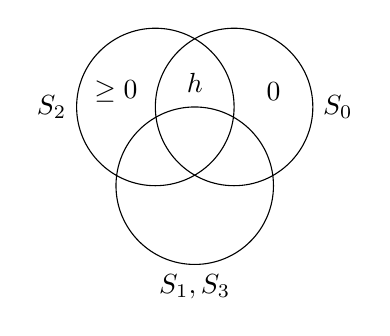
\begin{tikzpicture}
                \tikzstyle{circ}=[circle, draw, inner sep=0pt, minimum width=2cm]

                \node[circ, label=left:$S_2$]  (a) at (1,1) {};
                \node[circ, label=right:$S_0$]  (b) at (2,1) {};
                \node[circ, label=below:{$S_1, S_3$}] (c) at (1.5,0) {};
                \node at (0.5,1.2) {$\ge 0$};
                \node at (2.5,1.2) {$0$};
                \node at (1.5,1.3) {$h$};
            \end{tikzpicture}
        \end{center}
        Thus, $H(S_2 \mid S_1, S_3) \ge I(S_2 : S_0 \mid S_1, S_3) = h$.
    \end{proof}
\end{frame}
%%%%%%%%%%%%%%%%%%%%%%%%%%%%%%%%%%%%%%%%%%%%%%%%%%%%%%%%%%%%%%%%%%%%%%%%

%%%%%%%%%%%%%%%%%%%%%%%%%%%%%%%%%%%%%%%%%%%%%%%%%%%%%%%%%%%%%%%%%%%%%%%%
\begin{frame}{Ideal Secret Sharing Schemes: Lemma 2}
    \begin{lemma}
        $H(S_3 \mid S_1) \ge h$.
    \end{lemma}

    \begin{proof}
        Similarly to the previous lemma, we obtain that $H(S_3 \mid S_1, S_4) \ge h$, and consequently,
        $H(S_3 \mid S_1) \ge h$.
        \begin{center}
            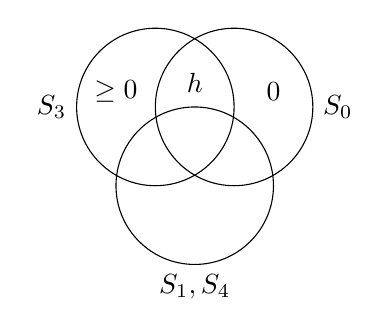
\begin{tikzpicture}
                \tikzstyle{circ}=[circle, draw, inner sep=0pt, minimum width=2cm]

                \node[circ, label=left:$S_3$]  (a) at (1,1) {};
                \node[circ, label=right:$S_0$]  (b) at (2,1) {};
                \node[circ, label=below:{$S_1, S_4$}] (c) at (1.5,0) {};
                \node at (0.5,1.2) {$\ge 0$};
                \node at (2.5,1.2) {$0$};
                \node at (1.5,1.3) {$h$};
            \end{tikzpicture}
        \end{center}
    \end{proof}
\end{frame}
%%%%%%%%%%%%%%%%%%%%%%%%%%%%%%%%%%%%%%%%%%%%%%%%%%%%%%%%%%%%%%%%%%%%%%%%



%%%%%%%%%%%%%%%%%%%%%%%%%%%%%%%%%%%%%%%%%%%%%%%%%%%%%%%%%%%%%%%%%%%%%%%%
\begin{frame}{Ideal Secret Sharing Schemes: Lemma 3}
    \begin{lemma}\label{lm:secret4:l3}
        $I(S_1 : S_3 \mid S_2) \ge h$.
    \end{lemma}

    \begin{proof}
        The following scheme should be interpreted as entropy conditioned on $S_2$.
        \begin{center}
            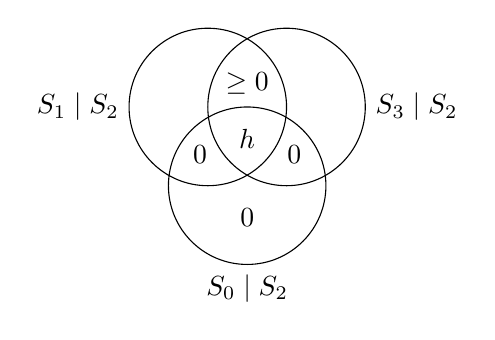
\begin{tikzpicture}
                \tikzstyle{circ}=[circle, draw, inner sep=0pt, minimum width=2cm]

                \node[circ, label=left: $S_1 \mid S_2$]  (a) at (1,1) {};
                \node[circ, label=right:$S_3 \mid S_2$]  (b) at (2,1) {};
                \node[circ, label=below:$S_0 \mid S_2$] (c) at (1.5,0) {};

                \node at (0.9,0.4) {$0$};
                \node at (1.5,1.3) {$\ge 0$};
                \node at (2.1,0.4) {$0$};

                \node at (1.5,-.4) {$0$};
                \node at (1.5,0.6) {$h$};
            \end{tikzpicture}
        \end{center}
        Note that $I(S_1 : S_0 \mid S_2) = h$ and $I(S_3 : S_0 \mid S_2) = h$, while
        $I(S_1 : S_0 \mid S_2, S_3) = 0$ and $I(S_3 : S_0 \mid S_1, S_2) = 0$.
        Thus, $I(S_1 : S_3 : S_0 \mid S_2) = h$, hence $I(S_1 : S_3 \mid S_2) \ge h$.
    \end{proof}
\end{frame}
%%%%%%%%%%%%%%%%%%%%%%%%%%%%%%%%%%%%%%%%%%%%%%%%%%%%%%%%%%%%%%%%%%%%%%%%

%%%%%%%%%%%%%%%%%%%%%%%%%%%%%%%%%%%%%%%%%%%%%%%%%%%%%%%%%%%%%%%%%%%%%%%%
\begin{frame}{Ideal Secret Sharing Schemes: Summing Up}
   \begin{proof}
            Now we just need to sum the results of the three lemmas:
        \[
        H(S_2) + H(S_3) \ge H(S_2, S_3) = H(S_2 \mid S_1, S_3) + H(S_3 \mid S_1) + I(S_1 : S_3 \mid S_2) +
        I(S_2 : S_1) \ge 3h.
        \]
  \end{proof}
\end{frame}
%%%%%%%%%%%%%%%%%%%%%%%%%%%%%%%%%%%%%%%%%%%%%%%%%%%%%%%%%%%%%%%%%%%%%%%%


%%%%%%%%%%%%%%%%%%%%%%%%%%%%%%%%%%%%%%%%%%%%%%%%%%%%%%%%%%%%%%%%%%%%%%%%
\begin{frame}{Lower Bound on Entropy of the Secret}
    \begin{theorem}[Csirmaz'94]
        There exist access structures $\Gamma$ on $n$ participants such that for any secret sharing scheme,
        $\max_i \frac{H(S_i)}{H(S_0)} \ge \Omega\left(\frac{n}{\log n}\right)$.
    \end{theorem}
\end{frame}
%%%%%%%%%%%%%%%%%%%%%%%%%%%%%%%%%%%%%%%%%%%%%%%%%%%%%%%%%%%%%%%%%%%%%%%%


\end{document}
